\documentclass[12pt]{article}

\usepackage{color}
\usepackage{nth}
\usepackage{enumitem}
\usepackage{booktabs}
\usepackage{tabularx}
\usepackage{hyperref}
\usepackage[pdftex]{graphicx}
\pagestyle{empty}
\setcounter{secnumdepth}{2}
\usepackage{float}

\pagestyle{empty}
\setcounter{secnumdepth}{2}

\topmargin=0cm
\oddsidemargin=0cm
\textheight=22.0cm
\textwidth=16cm
\parindent=0cm
\parskip=0.15cm
\topskip=0truecm
\raggedbottom
\abovedisplayskip=3mm
\belowdisplayskip=3mm
\abovedisplayshortskip=0mm
\belowdisplayshortskip=2mm
\normalbaselineskip=12pt
\normalbaselines

\begin{document}

\vspace*{0.5in}
\centerline{\bf\Large COMP 354}
\centerline{\bf\Large Design Document for myMoney}

\vspace*{0.5in}
\centerline{\bf\Large Team PA-PK}

\vspace*{0.5in}
\centerline{\today}

\vspace*{1.5in}
\begin{table}[htbp]
\caption{Team}
\begin{center}
\begin{tabular}{|r | c|}
\hline
Name & ID Number \\
\hline\hline
Anne-Laure Ehresmann & 27858906 \\
\hline
Marc-Antoine Dube & 40029307 \\
\hline
Kadeem Caines & 26343600 \\
\hline
Abdel Rahman Jawhar & 27192142 \\
\hline
Keith Dion & 40036340 \\
\hline
Hrachya Hakobyan & 40041555 \\
\hline
Andrew-Smith & 40034936 \\
\hline
Dongyu Chen & 27241909 \\
\hline
Yauheni Karaniuk & 40005680 \\
\hline
Renny Xu & 40005262\\
\hline
Wei Wang & 40041116 \\
\hline
\end{tabular}
\end{center}
\end{table}

\clearpage

\tableofcontents
\listoffigures
\listoftables

\clearpage


\section{Introduction and Purpose}

The goal of this document is to define the design for the desktop application myMoney. The majority of the design decisions have been taken     with the Requirements document in mind, one may thus want to look at this document first to have a clear picture of the problem in mind as well as the requirements demanded for the solution. This document presents an implementation of a possible solution to answer this problem. Its design is is outlined through an Architectural Design (AD), a Detailed design (DD) and Dynamic Design Scenarios (DDS) for the application. The AD focuses on high-level project decomposition, the DD describes the overarching system design (which includes the UML design, divided into multiple subsections), and the DDS displays how the subsystems interact with one another in order to produce system-level services. This document may thus be used to plan, coordinate, and guide the development of the software, estimate and allocate necessary resources for proper execution, and  then actually implement the software for the system. It seeks, above all, to serve as a precise and stable reference throughout the development.

\section{Scope}

This document contains everything to do with the development decisions and design of the system, all of which are derived from the requirements, which are not described in this document. Also not included in here is any testing of the system, which verifies that the requirements are met. It is merely a blueprint for a system that should, in theory, successfully pass any tests that would be done in correspondence with the requirements.

\section{Architectural Design} \label{sec:arch}

The myMoney application uses the Model-View-Controller (MVC) pattern to read, validate and modify the objects. The view is implemented through a JAVAFX front-end interface. This view then reports any events triggered by the user to the view controllers, which access the back-end and SQLite database to modify the model. Once updated, the model then passes its changes back to the view, to update the information displayed to the user. A more in-depth view of the interaction between the user and the view can be seen in the dynamic models, in section \ref{Dynamic Models}.

The controllers are implemented through a series of function calls to services which handle different layers of the application. All services perform their own validation, whether it is for implementing the business rules, or simply ensuring expected application behaviour (no null objects, caught exceptions...). Once this validation has been verified, the controllers passes the actually requested model change to the model. Examples of such services, their intercommunication, and their validation, is explained more in-depth in section \ref{subsystem interface}.

The model, which includes the back-end connection to the database, is the more complex part of the system. Lower layer services use the data access objects (DAO) to apply edits to the database, after the upper layers have verified the validity of the calls. Our system actually employs two databases; The first, a local database holding user info, bank account info, and transaction info, and the second, a "remote" database (also local, but acts as if it were remote) used to simulate the bank institutions' servers. When the user first adds a bank account, our view receives his input, passes it to the controls, which then makes requests for information to the "remote" database through the use of the services handling remote communication. These services receive a serialisation of the "remote" account, which it then translates into usable data for the local database. Once this has been successfully executed, the model triggers a view update, wherein the user can see his newly requested additions. All other events triggered by the user have no need of the remote database, and simply employ a series of communications between the controllers and the services handling local database. See section \ref{subsystem interface} for more details on these services and the databases.

\subsection{Architectural Diagram}

\begin{figure}[H]
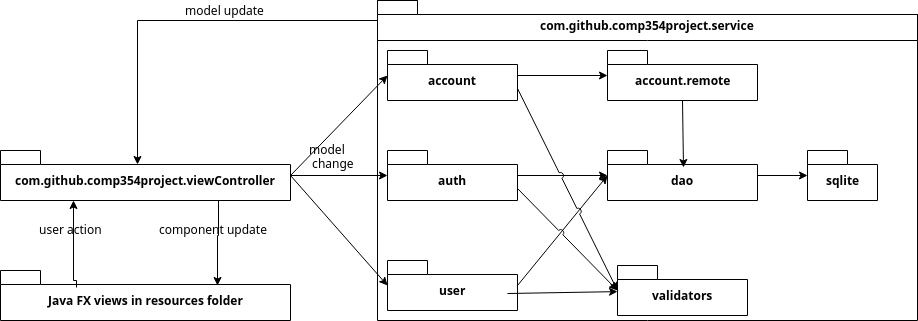
\includegraphics[width=\linewidth]{package-diagram.png}
\end{figure}

This design represents the MVC pattern discussed previously. The big advantage of this design is that everything is separated with interfaces which makes it easier to use different implementations, modify the features and create or mock tests.

The com.github.comp354project.service package is the main subsystem where most of the logic happens. The data validation and processing is done there. It connects to an SQLite database to persist the data. The com.github.comp354project.viewController calls this package to update the view and the model.

The com.github.comp354project.service package.account.remote package is a subsystem to our services which is meant to mock an API call to systems outside of ours like banks or credit card companies. Because we don't have access to these APIs for real, obviously, the data is persisted in the same SQLite database as the rest of the system.

\subsection{Subsystem Interface Specifications} \label{subsystem interface}

Specification of the software interfaces between the subsystems,
i.e. specific messages (or function calls) that are exchanged by the subsystems.
These are also often called ``Module Interface Specifications''.
Description of the parameters to be passed into these function calls in order to have a service fulfilled,
including valid and invalid ranges of values.
Each subsystem interface must be presented in a separate subsection.

*Note: The above is a description of what to provide. Need to edit into our own

\subsubsection{SignUpController Interfaces}

Below are the different models and services used in the SignUpController view.

\begin{figure}[H]
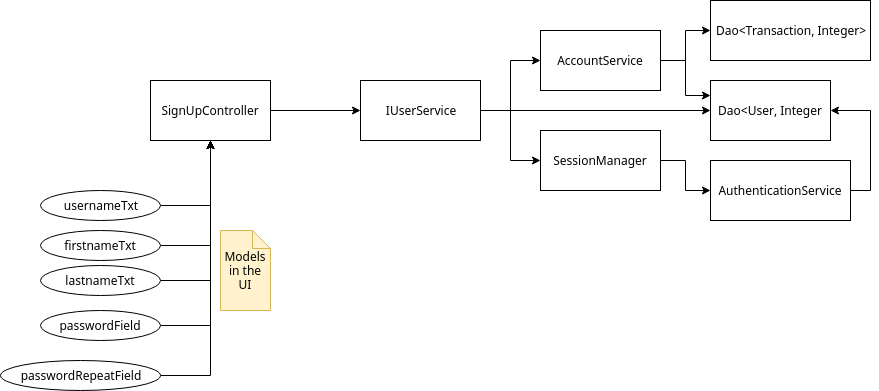
\includegraphics[width=\linewidth]{subsystem-interface-signup-controller.png}
\end{figure}

\clearpage

\subsubsection{LoginController Interfaces}

Below are the different models and services used in the LoginController view.

\begin{figure}[H]
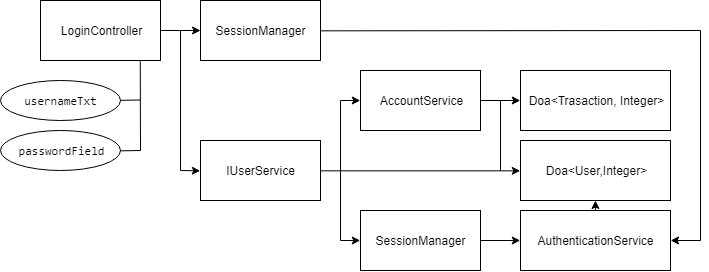
\includegraphics[width=\linewidth]{subsystem-interface-login-controller.png}
\end{figure}

\clearpage

\subsubsection{AcountDetailsController Interfaces}

Below are the different models and services used in the AccountDetailsController  view.

\begin{figure}[H]
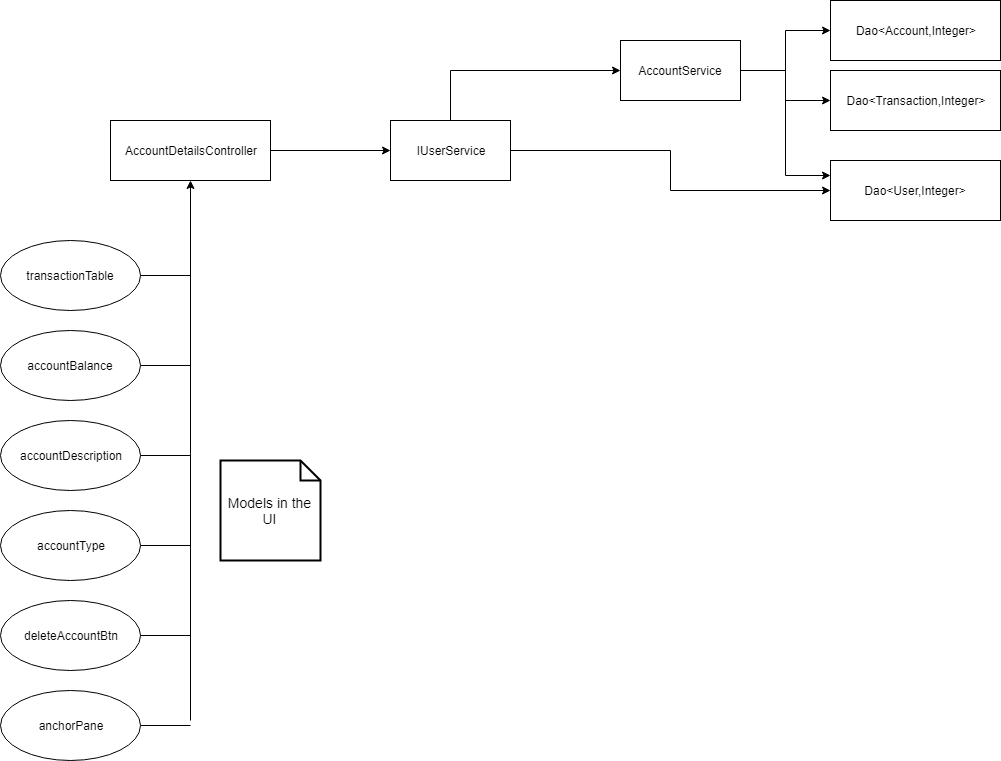
\includegraphics[width=\linewidth]{account-details-controller.png}
\end{figure}

\clearpage

\section{Detailed Design} \label{sec:detail}

The myMoney system architecture is designed to be easily modified because of the low coupling between the modules. This was done with interfaces and auto injection of dependencies in classes. Each service package has a Module class designed to bind and provide an implementation to an interface. This way, classes are never instantiated directly into each other, but injected. This design pattern is useful because a change in implementation is as simple as creating a new class and change the module binding. The classes that use it and the tests should in no way be changed. Mocking classes for test purposes is also much easier.

As a side note, we noticed that merge conflicts using git were much less likely to happen because we can each work on different parts of the system without modifying another module.

The tool used for this purpose is Dagger version 2.

\subsection{Class Diagram}

In this section we provide the class diagram of our system, useful for the system developers and testers.This is an in depth look at all of the classes within our system see figure \ref{fig:class-diagram} below If a term is unclear, view section \ref{glossary} for the glossary.

\begin{figure}[H]
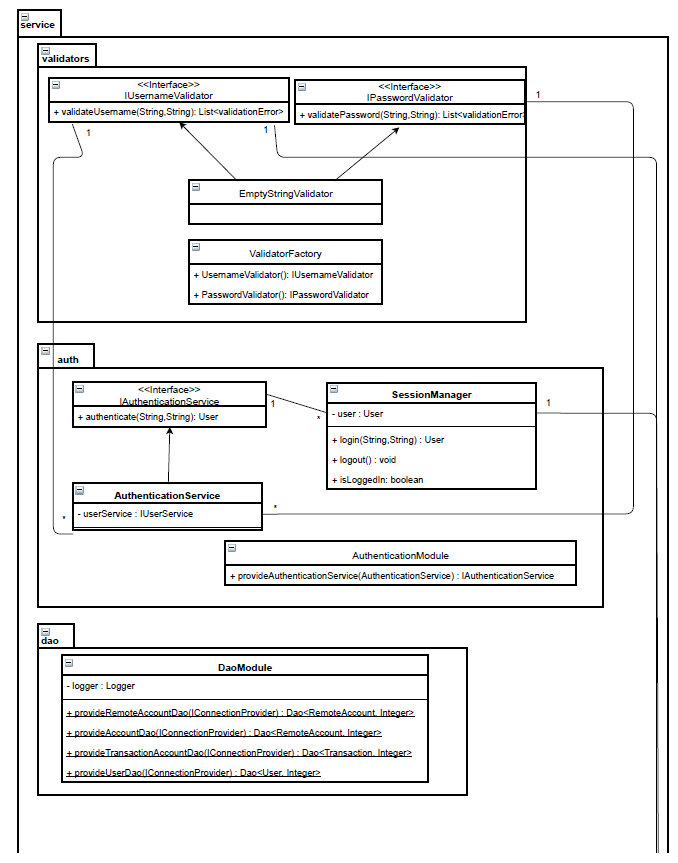
\includegraphics[width=\linewidth]{ClassDiagram1.png}
\end{figure}

\begin{figure}[H]
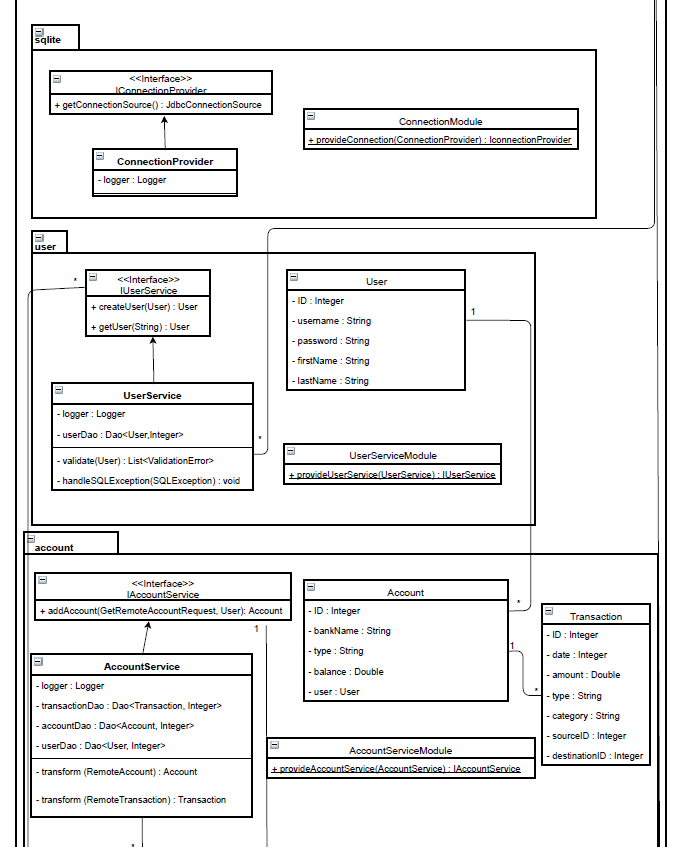
\includegraphics[width=\linewidth]{ClassDiagram2.png}
\end{figure}

\begin{figure}[H]
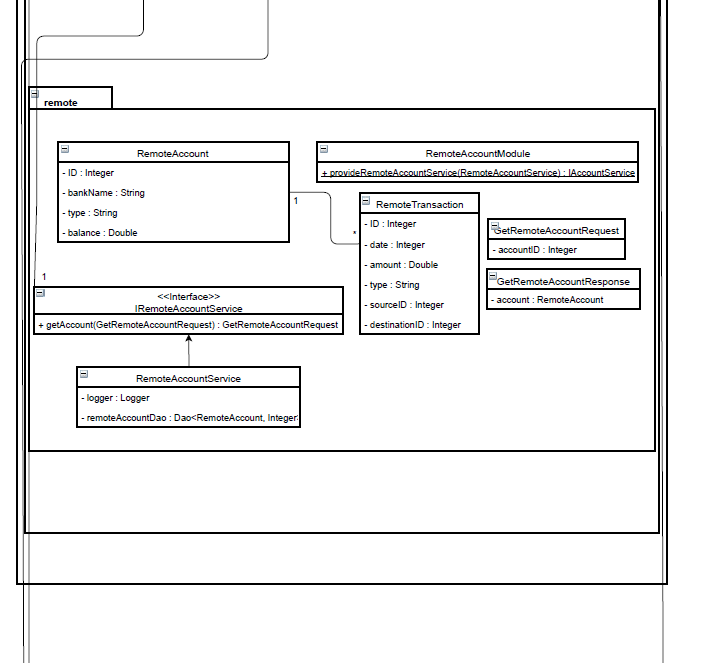
\includegraphics[width=\linewidth]{ClassDiagram3.png}
\end{figure}

\begin{figure}[H]
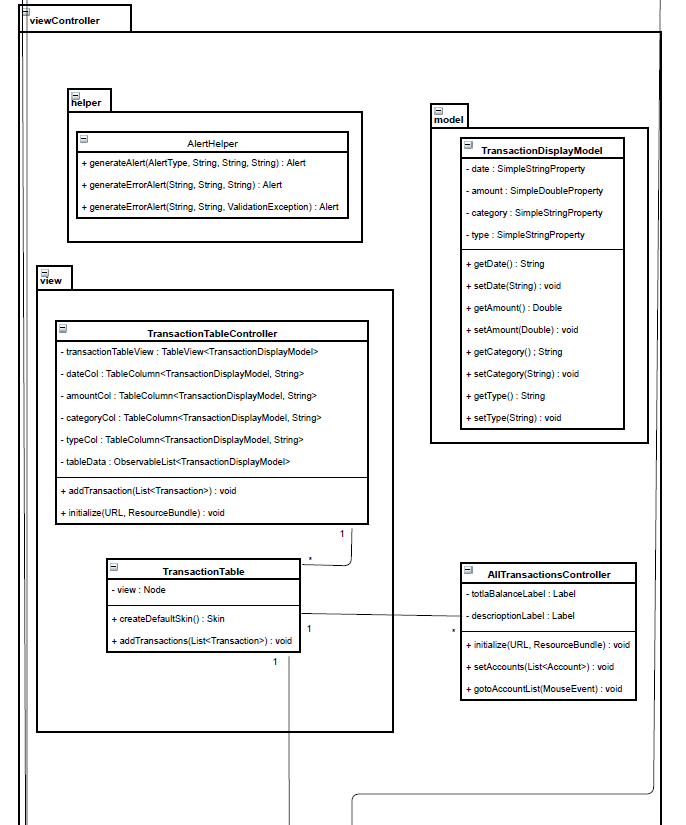
\includegraphics[width=\linewidth]{ClassDiagram4.png}
\end{figure}

\begin{figure}[H]
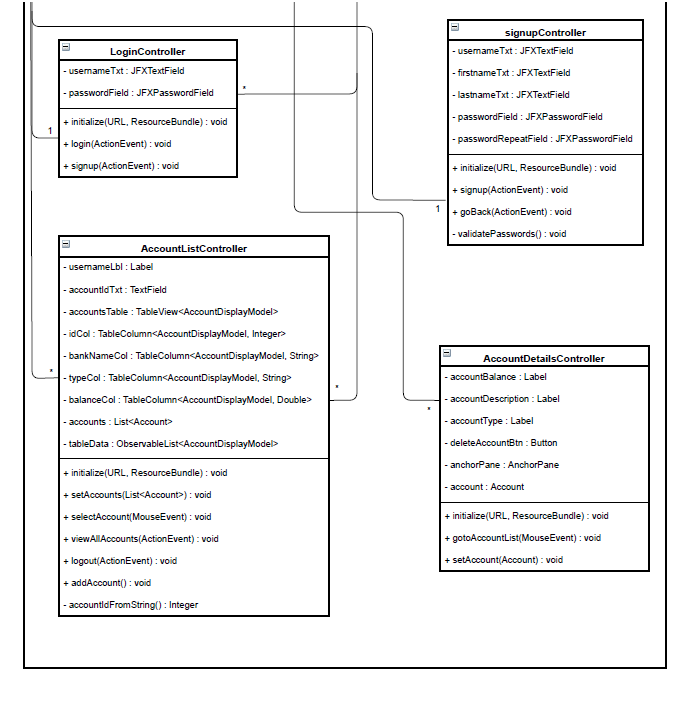
\includegraphics[width=\linewidth]{ClassDiagram5.png}
\caption{Class Diagram}
\label{fig:class-diagram}
\end{figure}


\clearpage

\subsection{Glossary of Domain Concepts} \label{glossary}
\begin{table}[H]
\caption{Glossary of Domain Concepts}
\begin{center}
\scalebox{0.7}{
\begin{tabular}{|l|p{0.8\linewidth}|}
\hline
Expression &  Definition \\
\hline
User & The person that is using the application and the main provider of requests to the system. \\
\hline
User Account & A data object containing user information. It also contains the various bank accounts that a user may have linked to the system. \\
\hline
Bank Account & A data object containing transactions linked with a specific bank account in a bank institution. One user account may have more than one bank accounts.\\
\hline
Transaction & Any kind of money exchange associated with a bank account.\\
\hline
Transfer & A type of transaction that occurs between two parties.\\
\hline
Deposit & A type of transaction where the owner puts money in his own bank account.\\
\hline
Withdrawal & A type of transaction where the owner of the bank account removes money from his balance.\\
\hline
Database & A local or online container which holds data in an organised, efficient manner. \\
\hline
Server & a computer that is accessible on a network, on which a database and/or system may be hosted. The bank institutions' databases will be hosted on here. \\
\hline
Object-Oriented Programming & A programming paradigm which separates entities into objects, and uses the concept of inheritance of properties, polymorphism of objects, encapsulation of objects. We use this paradigm for its maintainability and structural benefits.\\
\hline
MVC - Model-View-Controller Architecture & An architectural pattern which strictly separates components into the model (manages the data and logic), the view (output of the model), and the controller (handling input and passing it to the model or view).\\
\hline
Interface & A component of a system by which other entities (be it humans or other systems) may engage in an exchange of data with the system in question. \\
\hline
API - Application Programming Interface & A protocol or set of functions which serve as a method of communication to a software system. It is a type of interface, and the one by which our system will communicate with the banking institutions' databases. \\
\hline
DAO - Data access object & An object that provides an abstract interface to some type of database or other persistence mechanism.\\
\hline

\end{tabular}}
\end{center}
\end{table}

\clearpage

\subsection{Subsystem X}

\subsubsection{Detailed Design Diagram}

UML class diagram depicting the internal structure of the subsystem,
accompanied by a paragraph of text describing the rationale of this design.

*Note: The above is a description of what to provide. Need to edit into our own




\subsubsection{Units Description}

List each class in this subsystem and write a short description of its purpose,
as well as notes or reminders useful for the programmers who will implement them.
List all attributes and functions of the class.

*Note: The above is a description of what to provide. Need to edit into our own

\section{Dynamic Design Scenarios} \label{Dynamic Models}

Describe some (at least two) important execution scenarios of the system using UML sequence diagrams.
These scenarios must demonstrate how the various subsystems and units are interacting to achieve a system-level service.
Units and subsystems depicted here must be compatible with the descriptions provided in
section \ref{sec:arch} and \ref{sec:detail}.

*Note: The above is a description of what to provide. Need to edit into our own


\subsection{Dynamic Models of System Interface}

We have chosen 3 major functionalities of the system (also known as use cases) in order to portray the interactions between the classes of the system. By using a sequence diagram, this will display the dynamics visually by showcasing the sequences of method calls when a particular use case begins functioning.

\clearpage

\subsubsection{Use Case 1: Create User Account}

The following scenario depicts the actions that occur when a user clicks the sign up button in order to create their account. Firstly , the SignUpController (which represents the controller part of the MVC architecture) is called to handle the sign up event. The SignUpController then calls the validatePassword() method in order to check if the password chosen fits the required format. Next, the signupcontroller sends a message to the User class in order to start its builder method. The builder method is filled out with the info needed to sign up. The user class then sends a message to the IUserService class in order to finally create a user within the database using the information entered. Finally, the IUserService class calls the MyMoneyApplication's displayLogin() method in order to show the user the success of creating an account (The View)

\begin{figure}[H]
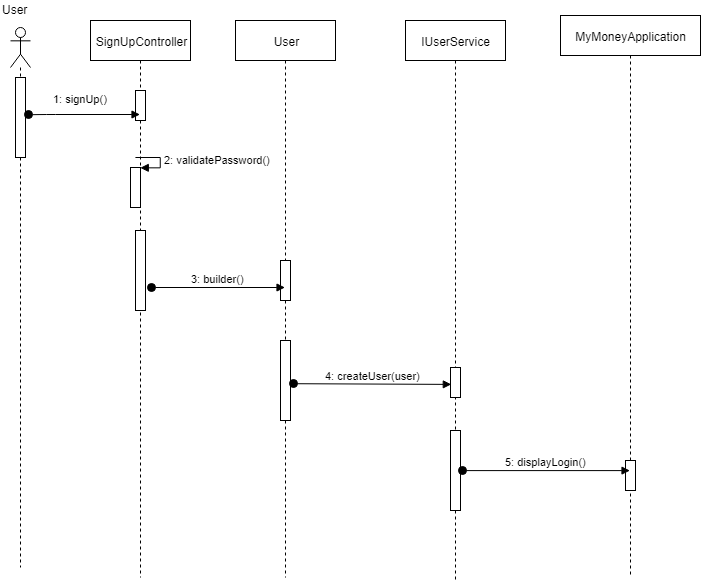
\includegraphics[width=\linewidth]{case1SequenceDiagram.png}
\caption{Use case 1 Sequence Diagram}
\label{fig:use-case-1-sequence-diagram}
\end{figure}

\clearpage

\subsubsection{Use Case 3: Add Bank Account to a User Account}

The following scenario describes the actions that occur when a user clicks the add button in the account list view.

\begin{figure}[H]
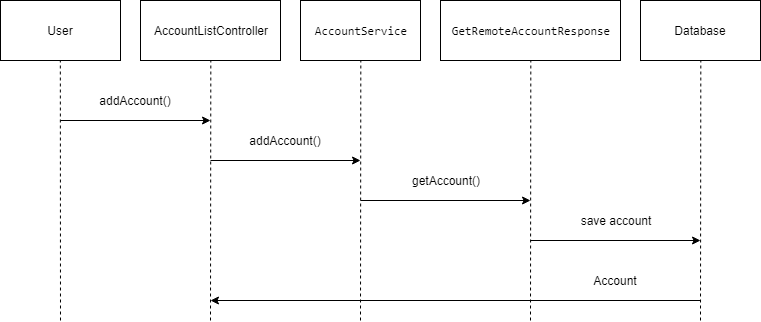
\includegraphics[width=\linewidth]{usecase3_sequence_diagram.png}
\caption{Use case 3 Sequence Diagram}
\label{fig:use-case-3-sequence-diagram}
\end{figure}

\clearpage

\subsubsection{Use Case 5: View Transactions for Specific Bank Account}

The following scenario describes the actions occur when user click the button<view transactions> for a specific bank account.

\begin{figure}[H]
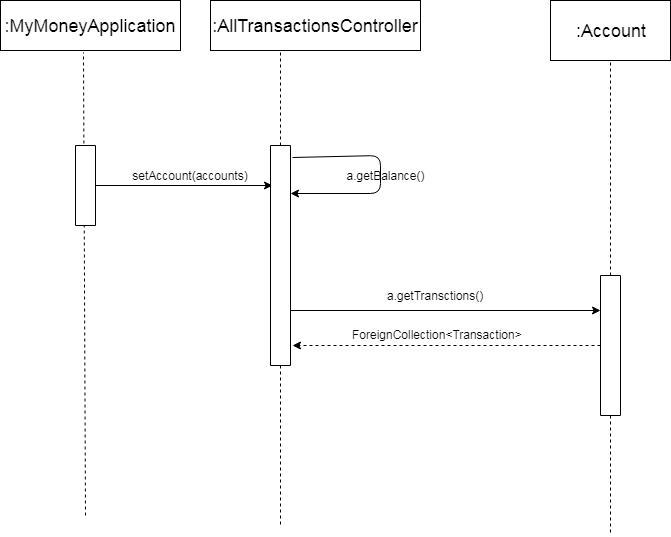
\includegraphics[width=\linewidth]{usecase5.png}
\caption{Use case 5 Sequence Diagram}
\label{fig:use-case-5-sequence-diagram}
\end{figure}

\clearpage

\clearpage

\subsubsection{Use Case 6: View All Transactions from all Bank Accounts}

The follwoing scenario describes the actions occur when user click the button<view all transactions> for viewsing all transactions from all bank accounts.

\begin{figure}[H]
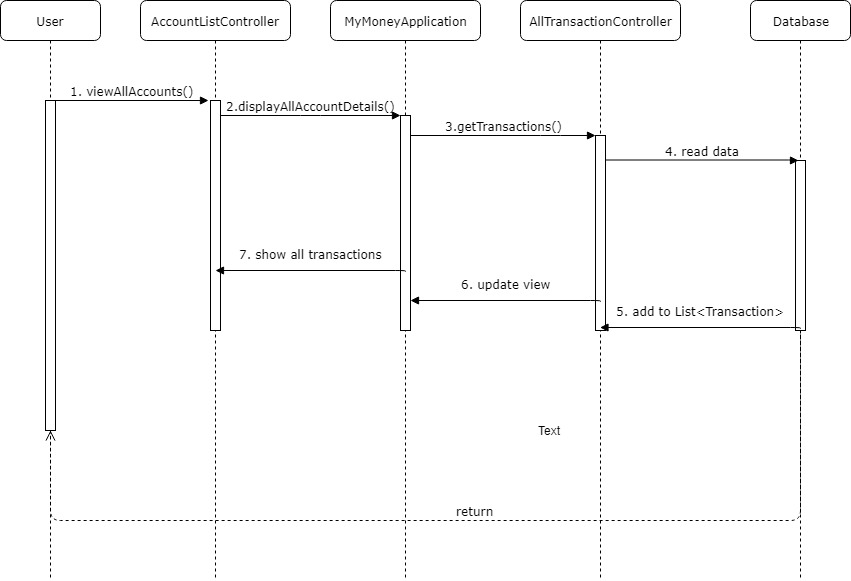
\includegraphics[width=\linewidth]{usecase6.jpg}
\caption{Use case 6 Sequence Diagram}
\label{fig:use-case-6-sequence-diagram}
\end{figure}

\clearpage

\section{Reference}

\begin{itemize}
\item User information: As our user and use-cases was based on feedback provided by our developers, our references lie mainly within our own team.
\item Craig Larman - Applying UML and Patterns
\item Greg Butler's course COMP 354 content
\item \href{http://web.mit.edu/ssit/cis/CISRequirements.html}{\textcolor{blue}{MIT Curricular Information System
Software Requirements Document}}
\item \href{https://resources.sei.cmu.edu/asset_files/TechnicalReport/2005_005_001_14621.pdf}{\textcolor{blue}{Carnegie Mellon Business Goals}}
\item \href{http://www.oracle.com/technetwork/testcontent/gettingstartedwithusecasemodeling-133857.pdf}{\textcolor{blue}{Use-Case: Oracle }}
\item \href{https://github.com/google/dagger}{\textcolor{blue}{Google Dagger Github}}

\end{itemize}

\end{document}
